Um die Elementarladung zu bestimmen, wird die Öltröpfenmethode verwendet. Es handelt sich dabei um eine Methode bei der ein Plattenkondensator, mit einem homogenen elektrischem Feld, in den mit einem Zerstäuber Öltröpfchen hineingegeben werden kann. Die Öltröpfchen sind dabei mit der Ladung $q$ geladen, $q$ entspricht einem vielfachen der Elementarladung. Ohne eingeschaltetem elektrischem Feld, lässt sich die Kräftegleichung schreiben als
\begin{align}
\frac{4\pi}{3}r^3\left( \rho_{\text{Öl}}-\rho_\text{L} \right)g=6\pi \eta_\text{L}rv_0.
\end{align}
Daraus lässt sich der Radius des Tröpfchens berechnen mit
\begin{align}
r=\sqrt{\frac{9\eta_\text{L}v_0}{2g\left( \rho_\text{Öl}-\rho_\text{L} \right)}}
\end{align}
\begin{figure}[h!]
\centering
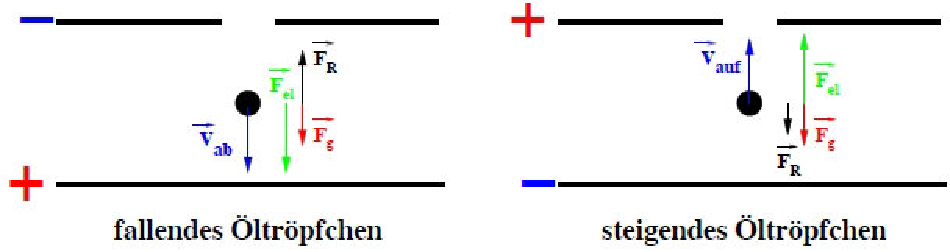
\includegraphics[scale=1]{Grafiken/Schema-Kondensator.pdf}
\caption{Die Kräfte auf das Tröpfchen mit eingeschaltetem elektrischem Feld \cite{V503}.\label{e-Feld}}
\end{figure}\\
Nach Abbildung \ref{e-Feld} lassen sich zwei Kräftegleichungen aufstellen.
\begin{align}
\frac{4\pi}{3}r^3\left( \rho_{\text{Öl}}-\rho_\text{L} \right)g-6\pi\eta_\text{L}rv_\text{ab}=-qE
\end{align}
und
\begin{align}
\frac{4\pi}{3}r^3\left( \rho_{\text{Öl}}+\rho_\text{L} \right)g+6\pi\eta_\text{L}rv_\text{auf}=+qE,
\end{align}
dabei sind $v_\text{ab}$ und $v_\text{auf}$ die Geschwindigkeiten, mit denen das Tröpfchen steigt beziehungsweise fällt. Aus den beiden Gleichungen folgt für die Ladung
\begin{align}
q=3\pi\eta_\text{L}\sqrt{\frac{9}{4}\frac{\eta_\text{L}}{g}\frac{(v_\text{ab}-v_\text{auf})}{(\rho_\text{Öl}-\rho_\text{L})}}\cdot\frac{(v_\text{ab}+v_\text{auf})}{E}
\end{align}
und für den Radius mit eingeschaltetem elektrischem Feld
\begin{align}
\label{eq:Theorie_Radius}
r=\sqrt{\frac{9\eta_\text{L}(v_\textbf{ab}-v_\text{auf})}{2g(\rho_\text{Öl}-\rho_\text{L})}}.
\end{align}
Bei diesen Gleichungen muss eine Korrektur durchgeführt werden, weil die Gleichungen nur für Tröpfchen gelten deren Abmessungen größer als die mittlere freie Weglänge in Luft ist.
Die Korrektur ist dabei gegeben als
\begin{align}
\label{eq:Theorie_Cunningham_Viskositaet}
\eta_\text{eff}=\eta_\text{L}\left( \frac{1}{1+B\frac{1}{pr}} \right),
\end{align}
sie wird als \textbf{Cunningham-Korrekturterm} bezeichnet und $B=6,17\cdot10^{-3}\, \text{Torr}\cdot \text{cm}$
Aus dieser folgt für die tatsächliche Ladung
\begin{equation}
\label{eq:Theorie_Cunningham_Ladung}
q^{\sfrac{2}{3}}= q_{0}^{\sfrac{2}{3}} \del{1+\dfrac{B}{pr}}.
\end{equation}